\newpage % Rozdziały zaczynamy od nowej strony.
\section{Warstwy}

\subsection{DENSE}
\subsection{CNN}
\subsection{LSTM}

% https://towardsdatascience.com/illustrated-guide-to-lstms-and-gru-s-a-step-by-step-explanation-44e9eb85bf21

\begin{figure}[!h]
    \label{fig:lstm_diagram}
    \centering 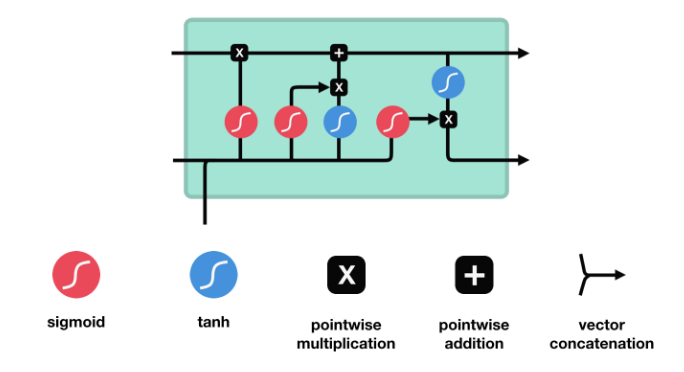
\includegraphics[width=1\linewidth]{lstm_diagram.png}
    \caption{Przepływ danych w jedynczym neuronie LSTM}
\end{figure}


\begin{figure}[!h]
    \label{fig:lstm_gates}
    \centering 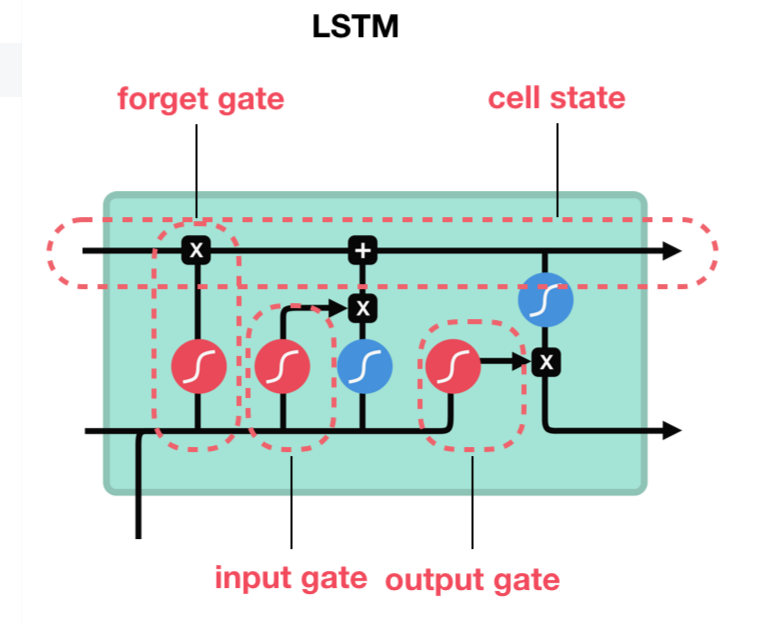
\includegraphics[width=0.5\linewidth]{lstm_gates.png}
    \caption{Przepływ danych w jedynczym neuronie LSTM}
\end{figure}


\subsubsection{Funkcje aktywacji}

Neuron LSTM wykorzystuje dwie funkcje aktywacji: 

\begin{itemize}
    \item Tahn (funkcja aktywacji typu tangens hiperboliczny) - pozwala ona na normalizowanie wektora tak by wartości zawierały się w ramach przedziału [-1,1] 
    \item Sigmoid (funkcja aktywacji sigmoidalna) - przekształca wartości wektora do wartości z przedziału [0,1]. Istotna z punktu widzenia określania, które elementy wektora powinny zostać zapamiętane (wartość bliżej 1), a które zapomniane (wartość bliżej 0) 
\end{itemize}


\subsubsection{Bramy}

W skład neuronu LSTM wchodzą następujące bramy: 


\subsection{Bi-LSTM}



 



 